\documentclass[11pt,a4paper]{article}
\usepackage[hyperref]{acl2019}
\usepackage{times}
\usepackage{latexsym}
\usepackage{smartdiagram}
\usepackage{url}
\usepackage{xcolor}
\usepackage{color}


\aclfinalcopy

\newcommand\BibTeX{B\textsc{ib}\TeX}
\title{\textit{Who wrote this : a framework for French novelist identification} \\
Machine Learning for Natural Language Processing 2020}

\author{Romain Avouac \\
  ENSAE  \\
  \texttt{romain.avouac@ensae.fr} \\\And
  Margot Eteve \\
  ENSAE \\
  \texttt{margot.eteve@ensae.fr} \\}

\setlength{\parindent}{0cm}
\date{}

\begin{document}
\maketitle

%%%%%%%%%%%%%%%%%%%%%%%%%%%%%%%%%%%%%%%%%%%%%%%%%%%%%%%%%%
% INTRODUCTION
%%%%%%%%%%%%%%%%%%%%%%%%%%%%%%%%%%%%%%%%%%%%%%%%%%%%%%%%%%
\section{Problem Framing}

Being able to identify authorship of a document is beneficial for a wide range of applications. It can prove very valuable from an historical perspective, since archives worldwide are full of documents whose authorship is not known with certainty. Furthermore, multiple plagiarism cases in literature could be solved with such an algorithm\footnote{See \href{https://en.wikipedia.org/wiki/Moli\%C3\%A8re_authorship_question}{here} and \href{https://en.wikipedia.org/wiki/Shakespeare_authorship_question}{here} for historical examples.}. Against that background, this project aims at developing a natural language processing (NLP) pipeline for authorship identification.

\section{Experiments Protocol}

\subsection{Data.} 

We choose to limit our experiment to a selection of ten French novelists from the 19th century\footnote{Zola, Maupassant, Daudet, Stendhal, Balzac, Flaubert, Hugo, Dumas, Vigny and Verne.}. Several reasons motivate this choice. First, the 19th century exhibits coherent and identifiable literary movements, whereas the 20th century literary is much more scattered for instance. Besides, the language used in 19th century books appears close enough to contemporary French, enabling the use of embeddings pre-trained on modern corpora. Finally, 19th century books are now in the public domain, and importantly directly available in digital format thanks to the \textit{Project Gutenberg}\footnote{\url{https://www.gutenberg.org/}}. For each author, three representative books have been selected : two for the training set and one for the test set. This clear separation between train and test sets ensures that we are not using a given book peculiarities (e.g character or place names) for prediction. Each book has been cut into paragraphs and each paragraph has been associated its author as label. This unit of analysis has been chosen because it is large enough that it can contain substantial statistical information and yet small enough that it can be processed easily by most NLP algorithms. The construction of the train and test sets can be fully reproduced using the scripts available in the GitHub repository of the project\footnote{\url{https://github.com/meteve/NLP_project}}.

\subsection{Preprocessing.} 

A major advantage of using data from the \textit{Project Gutenberg} is that it is highly normalized and virtually noiseless. It thus requires very little preprocessing to be directly usable in a machine learning pipeline. First, we perform a tokenization step. However, as we seek to distinguish authors based on their writing style, results can be highly sensitive to the choices made at this step. For instance, the amount of punctuation and the way it is used can be very distinctive of an author's style, yet it is generally removed by standard tokenizers. In order to ensure robustness of the results, we use various tokenization heuristics.

\subsection{Models.} 

We compare the performance of several models on the classification task. Our baseline consists in a linear classifier (logistic regression) trained on the TF-IDF weights matrix. All the other approaches we leverage are based on continuous word representations. The main challenge in this case is the computation of document vectors -- paragraph vectors in our case. Since there aren't actual theoretical guidelines to do so, we compare various models. First, we use a fully unsupervised technique: paragraph vectors are computed as a simple average of \verb|FastText| \cite{joulin2016bag} pre-trained French word vectors. Then we implement \verb|doc2vec| \cite{le2014distributed}, a supervised approach designed to learn word and document vectors jointly. For these two approaches, classification is also performed by training a linear classifier on the paragraph vectors matrix. Finally, we use the \verb|CamemBERT| model \cite{martin2019camembert}, a \verb|BERT| model pre-trained on a large French corpus. The model is fine-tuned in a supervised way through a simple dense layer with softmax activation.

\subsection{Evaluation.}  

We choose to evaluate our models with the F1 metric, which puts equal emphasis on both precision and recall. We also provide a more qualitative analysis of performance by analyzing the confusion matrix produced by our best classifier.

Both the NLP and the classification models are fine-tuned using grid search on a validation set which consists in half the test set. The other half is used for final evaluation.

\section{Results}

Performance comparison of the different models is presented in table~\ref{compar}. All the steps needed to reproduce these results are presented in a Colab notebook\footnote{\url{https://colab.research.google.com/drive/18Hj2zI-dL2YjCyW4vqPSkLYzNLRmk3wD}}. 

First, we observe that the TF-IDF approach is, as often, a strong baseline (F1 = 0.44). Since we deal with 10 classes, a random classifier would generate a F1 score of 0.1. Thus, TF-IDF results appear quite satisfactory for such a simple approach.  However, we notice that it tends to greatly overfit the training set (F1 = 0.9), likely because of the presence of peculiar character and place names which makes separation too easy on the training set. To support this intuition, we analyze the TF-IDF weights for the well-classified paragraphs of the training set for each author, and indeed find some character and place names in the top weights. We use Named Entity Recognition to detect and remove these elements. The F1 score on the training set is lower after removing the named entities (F1 = 0.82), but still high. Surprisingly, we find that the score on the validation set decreases (F1 = 0.42). The named entities seem to be relevant to identify authorship, since some characters and places can appear in multiple books. We thus decide to keep the proper nouns in the models.

Second, we observe substantial quality variation between the approaches based on continuous word representations. The FastText model performs the worst (F1 = 0.35), likely because it fails to take into account any context information due to the naive averaging procedure. The Doc2Vec model produces better results (F1 = 0.39), but still performs relatively poorly. On the contrary, the CamemBERT model exhibits much better performance (F1 = 0.5) and turns out to be the only approach which beats the TF-IDF baseline.



\begin{table}[]
\caption{Comparison of F1 scores on the test set}
\label{compar}
\begin{center}
\begin{tabular}{|l|l|}
\hline
\textbf{Model} & \textbf{F1 score} \\ \hline
CamemBERT       & 0.5                  \\ \hline
TF-IDF         & 0.44              \\ \hline
Doc2Vec        & 0.39                  \\ \hline
FastText      & 0.35                  \\ \hline
\end{tabular}
\end{center}
\end{table}

Finally, we notice a strong heterogeneity between authors through the analysis of the confusion matrix, displayed in figure~\ref{conf_matrix}. For instance, Dumas and Flaubert are generally well classified, both in terms of precision and recall. Some authors, such as Stendhal, exhibit a very high gap between the two metrics. Finally, Vigny appears to be the worst candidate for author identification, with both very poor precision and recall. This analysis suggests that some authors may have a more distinctive writing style than others.


\section{Discussion}

Our results show that it is possible, to a certain extent, to perform authorship identification of French 19th century novelists using NLP algorithms. However, we find that the performances of complicated deep learning approaches only come close  to those of a simple TF-IDF model with linear classification, which is disappointing. However, our study has important limitations. In particular, due to the high computational cost of fine-tuning the CamemBERT model, we had to set a maximum number of tokens per paragraph of 100, and we couldn't properly tune the learning rate. Without these limitations, it is likely that this approach would have produced more satisfactory results.

An idea for future works could be to use the tools of \textit{stylometry}\footnote{see \href{https://en.wikipedia.org/wiki/Stylometry}{here} for more details} -- which is used to attribute authorship in practice -- in order to build relevant features based on field knowledge. Such an approach could help to better distinguish authors based on their writing style.




%%%%%%%%%%%%%%%%%%%%%%%%%%%%%%%%%%%%%%%%%%%%%%%%%%%%%%%%%%
% DATA SELECTION
%%%%%%%%%%%%%%%%%%%%%%%%%%%%%%%%%%%%%%%%%%%%%%%%%%%%%%%%%%



\newpage

\bibliographystyle{plain}
\bibliography{biblio}

\bigskip

\section*{Appendix}

\begin{figure}[h]
\caption{Confusion matrix (CamemBERT)}
\label{conf_matrix}
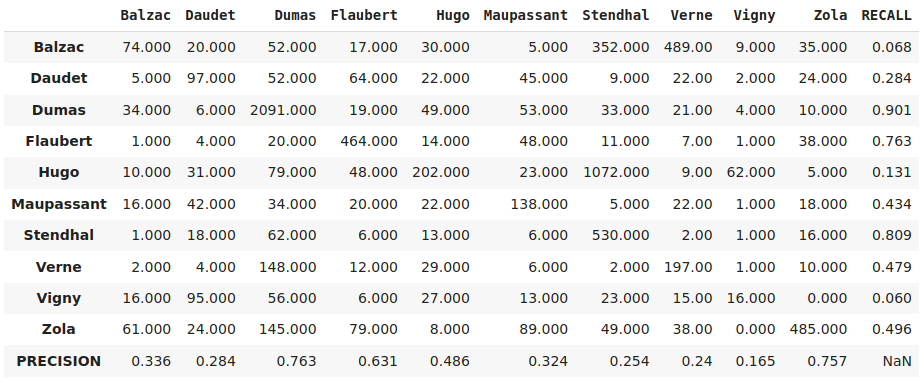
\includegraphics[scale=0.5]{figures/confusion.png}
\end{figure}




\end{document}